\documentclass{minimal}
\usepackage{bm}
\usepackage{epsfig,color}
\usepackage[papersize={576.00bp,432.00bp},text={576.00bp,432.00bp}]{geometry}
\begin{document}
\centering
% Title: glps_renderer figure
% Creator: GL2PS 1.3.8, (C) 1999-2012 C. Geuzaine
% For: Octave
% CreationDate: Fri Sep 25 13:40:27 2015
\setlength{\unitlength}{1pt}
\begin{picture}(0,0)
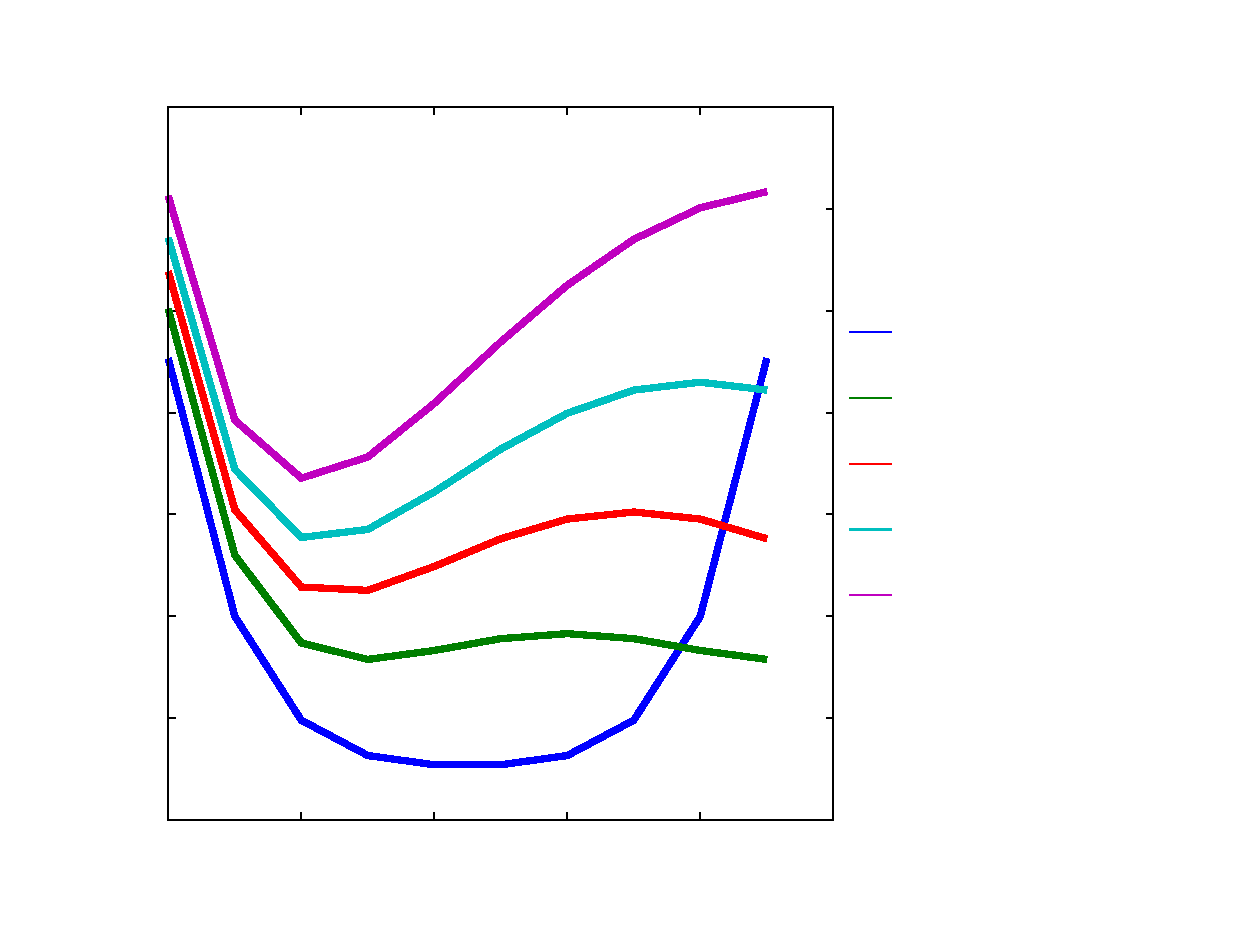
\includegraphics{proton_transfer_energy-inc}
\end{picture}%
\begin{picture}(576,432)(0,0)
\fontsize{16}{0}
\selectfont\put(72.7998,41.1855){\makebox(0,0)[t]{\textcolor[rgb]{0,0,0}{{0.8}}}}
\fontsize{16}{0}
\selectfont\put(136.632,41.1855){\makebox(0,0)[t]{\textcolor[rgb]{0,0,0}{{1}}}}
\fontsize{16}{0}
\selectfont\put(200.464,41.1855){\makebox(0,0)[t]{\textcolor[rgb]{0,0,0}{{1.2}}}}
\fontsize{16}{0}
\selectfont\put(264.297,41.1855){\makebox(0,0)[t]{\textcolor[rgb]{0,0,0}{{1.4}}}}
\fontsize{16}{0}
\selectfont\put(328.129,41.1855){\makebox(0,0)[t]{\textcolor[rgb]{0,0,0}{{1.6}}}}
\fontsize{16}{0}
\selectfont\put(391.961,41.1855){\makebox(0,0)[t]{\textcolor[rgb]{0,0,0}{{1.8}}}}
\fontsize{16}{0}
\selectfont\put(67.7974,46.1953){\makebox(0,0)[r]{\textcolor[rgb]{0,0,0}{{-4138.5}}}}
\fontsize{16}{0}
\selectfont\put(67.7974,95.0801){\makebox(0,0)[r]{\textcolor[rgb]{0,0,0}{{-4138}}}}
\fontsize{16}{0}
\selectfont\put(67.7974,143.991){\makebox(0,0)[r]{\textcolor[rgb]{0,0,0}{{-4137.5}}}}
\fontsize{16}{0}
\selectfont\put(67.7974,192.902){\makebox(0,0)[r]{\textcolor[rgb]{0,0,0}{{-4137}}}}
\fontsize{16}{0}
\selectfont\put(67.7974,241.787){\makebox(0,0)[r]{\textcolor[rgb]{0,0,0}{{-4136.5}}}}
\fontsize{16}{0}
\selectfont\put(67.7974,290.698){\makebox(0,0)[r]{\textcolor[rgb]{0,0,0}{{-4136}}}}
\fontsize{16}{0}
\selectfont\put(67.7974,339.583){\makebox(0,0)[r]{\textcolor[rgb]{0,0,0}{{-4135.5}}}}
\fontsize{16}{0}
\selectfont\put(67.7974,388.494){\makebox(0,0)[r]{\textcolor[rgb]{0,0,0}{{-4135}}}}
\fontsize{16}{0}
\selectfont\put(232.381,28.1865){\makebox(0,0)[t]{\textcolor[rgb]{0,0,0}{{Proton-oxygen distance [\AA]}}}}
\fontsize{16}{0}
\selectfont\put(26.7974,217.345){\rotatebox{90}{\makebox(0,0)[b]{\textcolor[rgb]{0,0,0}{{Energy [eV]}}}}}
\fontsize{16}{0}
\selectfont\put(422.661,280.689){\makebox(0,0)[l]{\textcolor[rgb]{0,0,0}{{$d_{OO} =2.5$ \AA}}}}
\fontsize{16}{0}
\selectfont\put(422.661,249.02){\makebox(0,0)[l]{\textcolor[rgb]{0,0,0}{{$d_{OO} = 2.8$ A}}}}
\fontsize{16}{0}
\selectfont\put(422.661,217.35){\makebox(0,0)[l]{\textcolor[rgb]{0,0,0}{{$d_{OO} = 3 $\AA}}}}
\fontsize{16}{0}
\selectfont\put(422.661,185.681){\makebox(0,0)[l]{\textcolor[rgb]{0,0,0}{{$d_{OO}=3.2$ \AA}}}}
\fontsize{16}{0}
\selectfont\put(422.661,154.011){\makebox(0,0)[l]{\textcolor[rgb]{0,0,0}{{$d_{OO} = 3.5$ \AA}}}}
\end{picture}
\end{document}
